\documentclass[tikz,border=10pt]{standalone}
\usepackage{pgfplots}
\pgfplotsset{compat=1.18}
\begin{document}
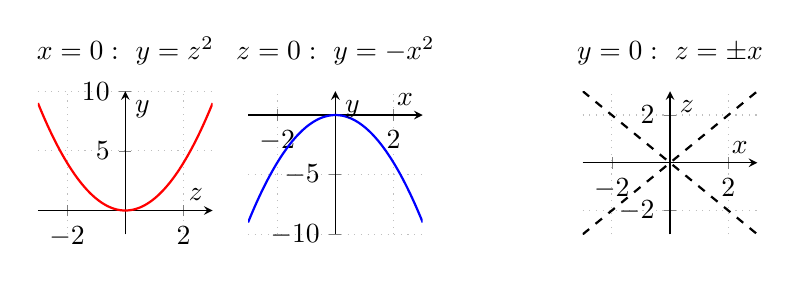
\begin{tikzpicture}
\begin{axis}[
    name=plot1,
    width=3.8cm, height=3.4cm,
    xlabel={$z$}, ylabel={$y$},
    title={$x=0:\ y=z^2$},
    grid=both,
    grid style={dotted},
    axis lines=middle,
    ymin=-2, ymax=10,
    xmin=-3, xmax=3
]
\addplot[domain=-3:3, samples=100, thick, red] {x^2};
\end{axis}

\begin{axis}[
    at={(plot1.east)}, anchor=west, xshift=0.45cm,
    width=3.8cm, height=3.4cm,
    xlabel={$x$}, ylabel={$y$},
    title={$z=0:\ y=-x^2$},
    grid=both,
    grid style={dotted},
    axis lines=middle,
    ymin=-10, ymax=2,
    xmin=-3, xmax=3
]
\addplot[domain=-3:3, samples=100, thick, blue] {-x^2};
\end{axis}

\begin{axis}[
    at={(plot1.east)}, anchor=west, xshift=4.7cm,
    width=3.8cm, height=3.4cm,
    xlabel={$x$}, ylabel={$z$},
    title={$y=0:\ z=\pm x$},
    grid=both,
    grid style={dotted},
    axis lines=middle,
    ymin=-3, ymax=3,
    xmin=-3, xmax=3
]
\addplot[domain=-3:3, samples=100, thick, black, dashed] {x};
\addplot[domain=-3:3, samples=100, thick, black, dashed] {-x};
\end{axis}
\end{tikzpicture}
\end{document}